\newpage
\section{计算机视觉与自然语言处理}

\subsection{生成: 图像}
\begin{enumerate}
    \item Variational AutoEncoder, VAE (变分自动编码器)
    \item Generative Adversarial Network, GAN (生成对抗网络)
    \item Diffusion Model
\end{enumerate}

\subsubsection{数据分布}
将一张 $H\times W\times 3$的图像看作 $3HW$维中的一点. 采样来自现实世界, 并不均匀分布到此空间中. 

\begin{figure}[!htb]
    \centering
    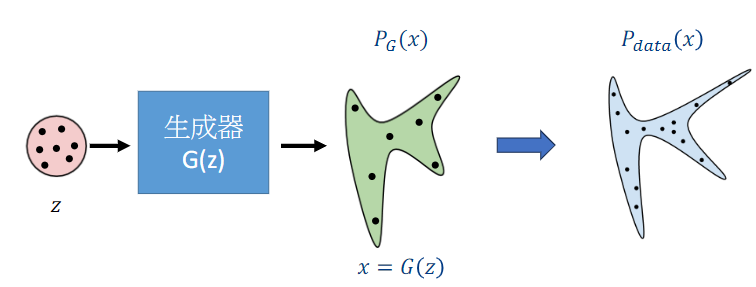
\includegraphics[width=0.42\textwidth]{pic/DL3/数据生成}
    \caption{数据分布看生成}
\end{figure}

从数据分布的角度看生成
\begin{align*}
    G^*=\arg \min_G Div(P_G, P_{data})
\end{align*}

\subsubsection{VAE}
AutoEncoder (自动编码器): 不具备生成功能, 仅作数据编解码

\begin{figure}[!htb]
    \centering
    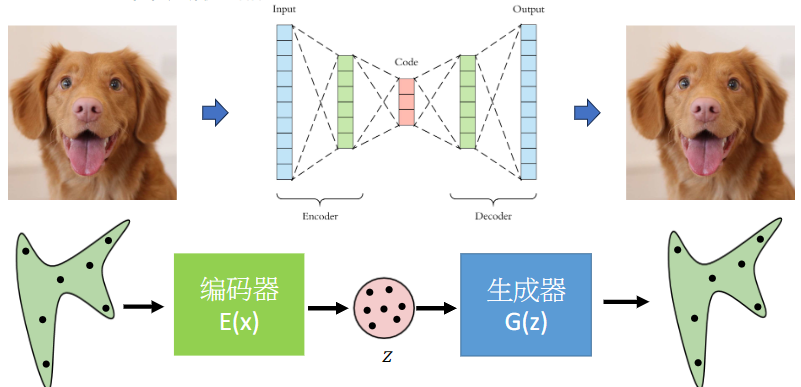
\includegraphics[width=0.42\textwidth]{pic/DL3/AutoEncoder}
    \caption{AutoEncoder}
\end{figure}

VAE: 加个噪声, 让一个点的特征能覆盖更多的编码空间, 这样采样编码空间时有更大机会采样出合理的特征. 

\begin{figure}[!htb]
    \centering
    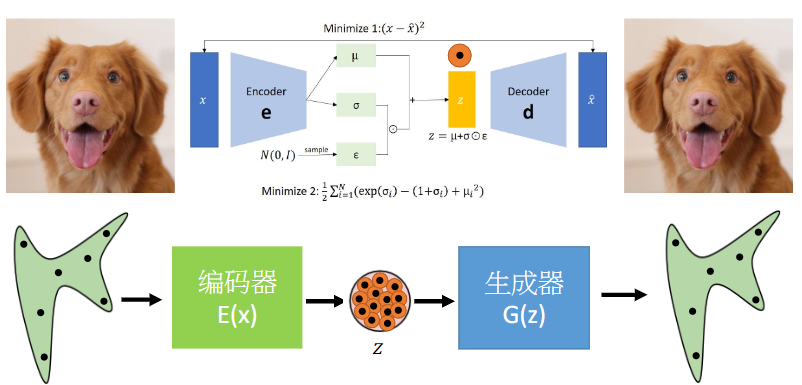
\includegraphics[width=0.42\textwidth]{pic/DL3/VAE}
    \caption{VAE}
\end{figure}

\subsubsection{GAN}
两个网络, 对抗训练

\subsubsection{Diffusion}
``近似''从高维空间采样
\begin{figure}[!htb]
    \centering
    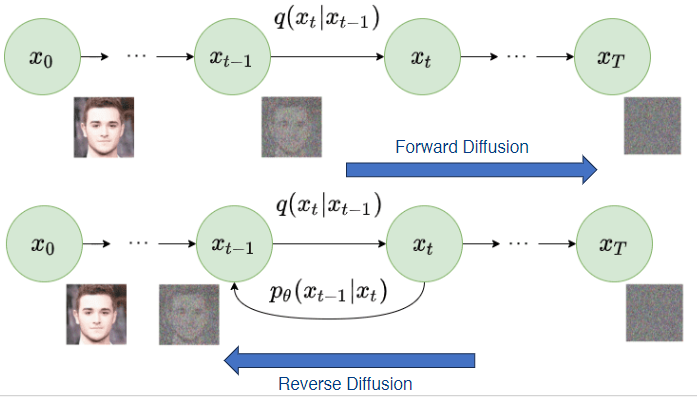
\includegraphics[width=0.42\textwidth]{pic/DL3/Diffusion}
    \caption{Diffusion}
\end{figure}

\subsection{其他任务}
\begin{enumerate}
    \item 机器翻译: 基于LSTM的机器翻译
    \item 分类: Vision Transformer
    \begin{figure}[!htb]
        \centering
        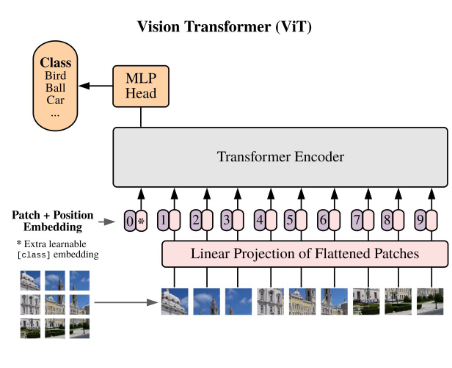
\includegraphics[width=0.309\textwidth]{pic/DL3/Vision Transformer}
        \caption{Vision Transformer}
    \end{figure}
    
    \item 语义分割: UNet
    \begin{figure}[!htb]
        \centering
        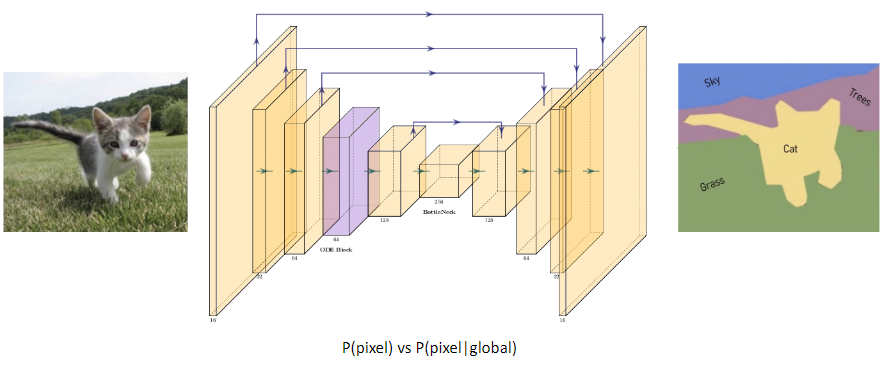
\includegraphics[width=0.309\textwidth]{pic/DL3/UNet.png}
        \caption{UNet}
    \end{figure}
    
    \item 无监督领域自适应: 行人重识别(person re-ID) 从容易到复杂
    \item 对比学习: CLIP (Contrastive Language-Image Pre-training)
    \begin{figure}[!htb]
        \centering
        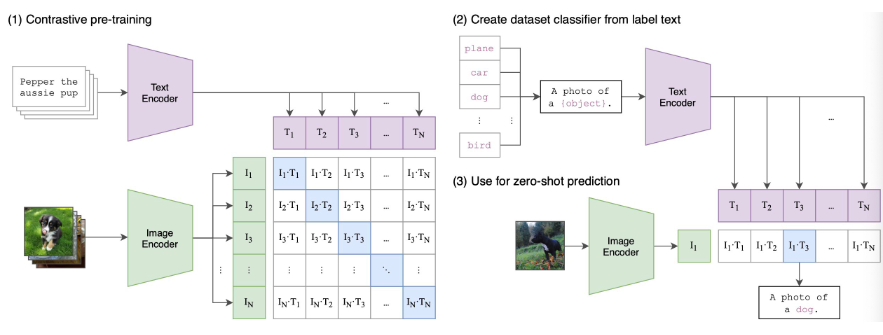
\includegraphics[width=0.42\textwidth]{pic/DL3/CLIP.png}
        \caption{CLIP}
    \end{figure}
    
    \item 自监督学习: MAE(Masked Autoencoder)
    \item 元学习: Meta-learning describes machine learning algorithms that acquire the knowledge and understanding from the outcome of other machine learning algorithms.
\end{enumerate}


\subsection{点云}
特征越深, 等价于分得越细
\begin{align*}
    F'^{(x,y,z)}=\max_{\| (\delta_x, \delta_y, \delta_z) \|\le r}MLP(F^{(x+\delta_x, y+\delta_y,z+\delta_z)}, (\delta_x, \delta_y, \delta_z))
\end{align*}